\documentclass{ieeetj}
\usepackage{cite}
\usepackage{amsmath,amssymb,amsfonts,amsthm,mathtools}
\usepackage{graphicx,color}
\usepackage{xcolor}
\usepackage{booktabs}
\usepackage{multirow}
\usepackage{url}
\usepackage{bm}
\usepackage{siunitx}
\usepackage{algorithm}
\usepackage{algpseudocode}
\usepackage{hyperref}
\hypersetup{hidelinks=true}
\setlength{\textfloatsep}{1.0\baselineskip plus 0.2\baselineskip minus 0.3\baselineskip}
\setlength{\dbltextfloatsep}{1.0\baselineskip plus 0.2\baselineskip minus 0.3\baselineskip}
\setlength{\floatsep}{0.8\baselineskip plus 0.2\baselineskip minus 0.2\baselineskip}
\setlength{\dblfloatsep}{0.8\baselineskip plus 0.2\baselineskip minus 0.2\baselineskip}
\AtBeginDocument{\definecolor{tmlcncolor}{cmyk}{0.93,0.59,0.15,0.02}\definecolor{NavyBlue}{RGB}{0,86,125}}

\makeatletter
\let\@revised\@empty
\makeatother

% The class numbers a subsection as a bare letter, so every \ref to a subsection
% printed as "Section B" with no section number, and two different subsections
% both printed as "Section B". Restore the section number, which is the form
% IEEE uses in running text.
\renewcommand{\thesubsection}{\thesection\text{-}\Alph{subsection}}

% Two full width floats landed together on a page of their own, which cost a
% whole page of text. These are the standard float parameters, loosened so a
% page carrying a wide float still carries body text.
\renewcommand{\textfraction}{0.07}
\renewcommand{\topfraction}{0.92}
\renewcommand{\bottomfraction}{0.92}
\renewcommand{\dbltopfraction}{0.92}
\renewcommand{\floatpagefraction}{0.80}
\renewcommand{\dblfloatpagefraction}{0.80}
\setcounter{topnumber}{3}
\setcounter{dbltopnumber}{2}
\setcounter{totalnumber}{4}
% allow a full width float at the foot of a page, so the wide table and the
% wide figure can share one page instead of taking one each
\usepackage{stfloats}

\def\BibTeX{{\rm B\kern-.05em{\sc i\kern-.025em b}\kern-.08em
    T\kern-.1667em\lower.7ex\hbox{E}\kern-.125emX}}
\def\OJlogo{}
\def\seclogo{}
\def\authorrefmark#1{\ensuremath{^{\textbf{#1}}}}
\newtheorem{theorem}{Theorem}
\newtheorem{corollary}{Corollary}
\newtheorem{definition}{Definition}

% Numbers measured by revision/diagnostics.py, regenerated by revision/make_tables.py.
% generated from diagnostics_nafnet.json over 173 images
\newcommand{\LipTheory}{0.5489}
\newcommand{\LipMeasured}{0.4679}
\newcommand{\AllocMean}{0.727}
\newcommand{\AllocStd}{0.050}
\newcommand{\NImages}{173}
\newcommand{\CondMargin}{141}
\newcommand{\CondSigma}{147}
\newcommand{\BoundOK}{99}
\newcommand{\CalibRho}{-0.258}
\newcommand{\CalibAuse}{0.775}
\newcommand{\EdgeInvBack}{0.45}
\newcommand{\EdgeInvCorr}{0.49}
\newcommand{\WeakRetBack}{40.5}
\newcommand{\WeakRetCorr}{44.5}
\newcommand{\DarkFrac}{1.6}
\newcommand{\DarkChange}{0.0072}
\newcommand{\IlmShiftBack}{4.73}
\newcommand{\IlmShiftCorr}{4.28}
\newcommand{\RpeShiftBack}{9.93}
\newcommand{\RpeShiftCorr}{10.24}
\newcommand{\GlobalChange}{0.0107}
\newcommand{\AllocMin}{0.556}
\newcommand{\AllocMax}{0.794}
\newcommand{\AllocClamp}{0.00}
\newcommand{\SigmaRatio}{0.961}
\newcommand{\EtaT}{0.0010}
\newcommand{\EtaB}{-0.0003}



\begin{document}
% วันที่ได้รับอนุมานจากหมายเลขต้นฉบับ OJCS-2026-04-0386 ซึ่งระบุเดือนเมษายน 2026
% และจากวันที่ของไฟล์ที่ส่ง ต้องยืนยันกับอีเมลตอบรับจากวารสารก่อนส่ง
\receiveddate{}
\reviseddate{}
\accepteddate{}
\publisheddate{}
\currentdate{}
\doiinfo{}
\markboth{}{Anonymous et al.}
\title{Backbone-Modular Neuro-Symbolic Post-Correction for OCT Denoising via Explicit Predicate Maps and Stable Fuzzy Allocation}
\author{Anonymous Author(s)\authorrefmark{1}}
\affil{\authorrefmark{1} Anonymous Affiliation}
\corresp{Correspondence withheld for double blind review.}

\begin{abstract}
Denoisers for optical coherence tomography are trained to reduce a pixel error, so they can raise
fidelity while lowering what a clinician reads, the contrast between retinal layers and the sharpness
of their boundaries. We repair those properties afterwards, leaving the denoiser untouched. A
small wrapper on the frozen denoiser measures six named clinical properties from the noisy input and
its output alone, needing no clean image at test time, turns them into a per-pixel decision through five rules in fuzzy
logic, bounds how far the image may move, and keeps a proposed change only while stated constraints
hold, so every change is attributable to a named property at a named place. We prove that the decision cannot jump, by an exact rather than a loose constant, and give
conditions under which the correction cannot lower contrast. One set of rules, budgets
and weights serves four denoisers, only a small head being refitted. On all four, contrast
rises by 3.5 to 11.3 percent and speckle suppression by 23.7 to 57.1 percent, for 0.17 to 0.98 dB of
fidelity, and 21 of 24 gains clear the spread across seeds. Carried unchanged to two further datasets,
40 of 48 pairs improve.
\end{abstract}

\begin{IEEEkeywords}
Clinical quality assessment, fuzzy logic, image denoising, neuro-symbolic reasoning, optical
coherence tomography.
\end{IEEEkeywords}

\maketitle

\section{Introduction}
\label{sec:introduction}
\IEEEPARstart{O}{ptical} coherence tomography (OCT) is the standard non invasive way to image the
retina~\cite{huang1991optical}. Every OCT image carries speckle, a multiplicative disturbance that
arises from coherent light scattering inside tissue~\cite{goodman2007speckle}. Speckle blurs the
border between retinal layers, lowers the contrast between tissue and background, and makes
automatic layer segmentation less reliable~\cite{devalla2018drunet}.

Deep denoisers remove much of that disturbance, but they are almost always trained to minimise the
squared error against a clean reference, so a denoiser can raise the peak signal to noise ratio (PSNR)
of a scan while making it less useful to a clinician. Layer boundaries lose definition, the contrast
between tissue and the dark vitreous falls, and thin structures with weak signal fade into the
background. None of these losses is visible in a PSNR number, and none is corrected by training the
same objective harder.

\subsection{Motivation}
The gap we address is not a missing denoiser. It is that nothing sits between the denoiser and the
clinical reader to state in explicit terms what a good OCT image should look like and to repair the
specific ways in which a denoised image falls short. Building that part as another neural block would
hide the reason for every change inside learned weights again, while a clinician, a regulator or a
reviewer who sees a modified scan needs to know which property was judged deficient, where that
judgement was made, and how large a change was allowed. This paper therefore treats post correction as
its own problem. We keep the denoiser frozen and attach a small policy, written as named image
properties, explicit logical rules over them, and explicit limits on the size of any change, that
decides where the image should change and by how much. Every learned map in the decision path is
bounded, and its effect reaches the image only through a named rule.

\subsection{New ideas in this paper}
\label{sec:contributions}
The new ideas are three, and we do not claim that edge filters, gating maps or fuzzy operators are
new on their own.

\begin{enumerate}
\item \textbf{Six clinical properties given in closed form.}
Section~\ref{sec:predicates} defines six predicates that need no ground truth. Each returns a score
for the whole image and a map of where the property is unsatisfied. Both are formulas, so the input
to the rule layer can be recomputed by anyone from the released code.

\item \textbf{A fuzzy allocation rule with a proved and measured sensitivity bound.}
Section~\ref{sec:negotiator} builds the allocation from Lukasiewicz connectives.
Section~\ref{sec:stability} defines what stability means here and proves a Lipschitz bound, and
Section~\ref{sec:theory_check} measures the true sensitivity on real images and compares it with the
bound. A bound that is never checked against data is a claim, not a guarantee.

\item \textbf{A safety layer that decides how much of a proposal to keep.}
Section~\ref{sec:safety} states three constraints at three scales and shows how the number of
satisfied constraints sets the fraction of the proposed change that is applied. A margin condition
under which the correction cannot lower the contrast to noise ratio is proved and then tested
numerically.
\end{enumerate}


\section{Related Work}
\label{sec:related}

\subsection{Denoising of OCT images}
Learned denoisers for OCT fall into three families. Convolutional networks such as
DnCNN~\cite{zhang2017beyond} and DRUNET~\cite{devalla2018drunet} learn a residual between the noisy
and the clean image. Attention based designs such as NAFNet~\cite{chen2022simple} and
KBNet~\cite{zhang2023kbnet} reweight features before combining them. Transformer designs such as
SwinIR~\cite{liang2021swinir} use windowed self attention. Classical estimators remain in use,
including non local means~\cite{buades2005non} and wavelet shrinkage~\cite{mayer2012wavelet}, and
self supervised training removes the need for clean targets~\cite{krull2019noise2void}. Methods
built for OCT address the scarcity of paired data directly, through triplet cross
fusion~\cite{geng2022triplet} and through sparse representation~\cite{fang2012sparsity,fang2013fast}.

All of these methods are trained to reduce a pixel error, so the quantity they optimise is not the
quantity a clinician reads. Work on automated quality assessment for
OCT~\cite{wang2019quality,stein2006quality,tewarie2012oscar} measures clinical quality but does not
act on it. The present paper closes that loop by turning measured quality into a correction applied
under stated limits.

\subsection{Confidence and uncertainty in medical imaging}
Dropout as an approximate Bayesian posterior~\cite{gal2016dropout}, task weighting driven by learned
variance~\cite{kendall2018multi} and deep ensembles~\cite{lakshminarayanan2017simple} are the
standard ways to attach a confidence to a prediction, and in OCT such values flag unreliable layer
segmentation~\cite{devalla2018drunet} and poor scan quality~\cite{wang2019quality}. In almost all of
that work the value is reported and then left alone, marking a region as doubtful without changing
what happens there. We instead feed such a map into the correction decision, and
Section~\ref{sec:confidence_check} reports that the map we built is not a confidence in this sense.

\subsection{Symbolic reasoning and expert networks joined with neural networks}
Neuro symbolic computing~\cite{garcez2023neurosymbolic} couples a learned model with explicit rules,
and differentiable fuzzy logic makes the coupling trainable because the connectives become smooth
functions of continuous truth values~\cite{vankrieken2022analyzing}. In medical imaging the pattern
has generated spinal reports by pairing a generative network with a symbolic graph of domain
knowledge~\cite{han2021unifying}, predicted patient deterioration with a probabilistic logic program
over convolutional features~\cite{fadja2022neural}, and interpreted corneal topography through a
knowledge graph attached to a learned feature model~\cite{wang2026explainable}. Fuzzy membership
functions have been embedded inside networks that process OCT directly, where a rough fuzzy
discretisation guides layer segmentation~\cite{chen2023deep}, and pixel level fuzzy rules have
replaced a learned attention block so that the resulting map reads as a logical
statement~\cite{kim2025pixel}.

A parallel line builds an image model from cooperating experts. Steered mixtures of experts combine
local regressors through an explicit steering term~\cite{ozkan2023steered}, also for OCT speckle
removal~\cite{ozkan2024denoising}, and recent restoration networks route an input through experts of
different capacity according to its difficulty~\cite{zamfir2025complexity}. Outside imaging, evolving
fuzzy models identify actuator dynamics from data~\cite{precup2021evolving}, learned models are
combined with a physical forward operator in ultrasound computed tomography~\cite{fan2022model}, and
the sensitivity of a differential model to its initial conditions is treated as a source of
uncertainty in simulation~\cite{casquilho2025effect}. All of these rest on the principle we rely on,
that a learned component becomes easier to trust when part of the decision is written in a language a
person can read. What is still missing is a rule layer that acts on the output of a strong denoiser,
names the clinical properties it protects, and limits how far it may move the image. That is the
object studied here.

\section{Notation and Problem Statement}
\label{sec:problem}

This section fixes the notation used in the rest of the paper and states the problem that the
method solves. Every symbol is defined here before it is used anywhere else.

\subsection{Notation}
\label{sec:notation}
Images are real valued arrays of height $H$ and width $W$ with values in $[0,1]$. We write $\mathbf{y}$
for the noisy B scan that comes off the scanner and $\mathbf{x}$ for the clean reference obtained by
averaging many repeated scans of the same location. A pixel index is written $p$, so $y_p$ is one
pixel of $\mathbf{y}$.

Two products appear. The symbol $\odot$ is the Hadamard product, which multiplies two arrays of the
same shape entry by entry, so $(\mathbf{a} \odot \mathbf{b})_p = a_p b_p$. Ordinary multiplication of
two numbers is written by juxtaposition with no symbol between the factors. Table~\ref{tab:notation}
lists every remaining symbol in the order in which the paper introduces it.

\begin{table}[!tb]
\centering
\caption{Symbols used in the paper, in order of first use.}
\label{tab:notation}
\setlength{\tabcolsep}{4pt}
\footnotesize
\begin{tabular}{lp{0.62\columnwidth}}
\toprule
Symbol & Meaning \\
\midrule
$\mathbf{y}$ & Noisy input B scan \\
$\mathbf{x}$ & Clean reference B scan \\
$f_\theta$ & Frozen denoising backbone with parameters $\theta$ \\
$\mathbf{b}$ & Backbone output, $\mathbf{b} = f_\theta(\mathbf{y})$ \\
$\phi$ & Trainable parameters of the wrapper \\
$\mathbf{z}$ & Backbone feature map read by the confidence head \\
$\mathbf{c}$ & Confidence map with values in $[0,1]$ \\
$\mathbf{u}$ & Uncertainty map, $\mathbf{u} = \mathbf{1} - \mathbf{c}$ \\
$s_i$ & Score of clinical property $i$, a number in $[0,1]$ \\
$\mathbf{m}_i$ & Failure map of clinical property $i$, values in $[0,1]$ \\
$\tau_i$ & Decision threshold for property $i$ \\
$f_i$ & Soft failure signal derived from $s_i$ and $\tau_i$ \\
$\boldsymbol{\Delta}$ & Raw multiplicative gain proposed by the gain network \\
$\boldsymbol{\lambda}$ & Per pixel strength map with values in $[0,1]$ \\
$\mathbf{a}$ & Allocation map produced by the rule layer \\
$\boldsymbol{\alpha}$ & Gain after allocation, strength and clamping \\
$\mathbf{g}$ & Intensity gate that suppresses change in the background \\
$\boldsymbol{\delta}_{\mathrm{e}}$ & Additive edge correction \\
$\mathbf{q}$ & Candidate image before the safety decision \\
$n$ & Number of satisfied safety constraints, an integer in $\{0,1,2,3\}$ \\
$w$ & Blend weight chosen from $n$ \\
$\hat{\mathbf{x}}$ & Final output of the wrapper \\
$\mathcal{T},\mathcal{B}$ & Sets of tissue pixels and background pixels \\
$\mu_\mathcal{T},\mu_\mathcal{B}$ & Mean value over tissue and over background \\
$\sigma_\mathcal{B}$ & Standard deviation over background \\
\bottomrule
\end{tabular}
\end{table}

\subsection{The optimisation problem}
The denoiser is given and is not changed. The task is to produce an image that beats
$\mathbf{b} = f_\theta(\mathbf{y})$ on named clinical measures, stays close to it everywhere, and can
explain every change it makes.
\label{sec:optimisation}
We now state the problem in the form that the training procedure actually solves. This makes precise
what is being optimised, over what, and subject to what.

\textbf{Decision variables.} The only free quantities are the wrapper parameters $\phi$. These are the
confidence head, the gain network, the edge network, the strength predictor and the rule layer. The
backbone parameters $\theta$ are held fixed throughout.

\textbf{Objective.} Let $\mathcal{D}$ be a set of paired scans. Let $\hat{\mathbf{x}}(\phi)$ be the
output of the wrapper. We minimise the expected value of a weighted sum of five terms,
\begin{equation}
\min_{\phi}\;\; \mathbb{E}_{(\mathbf{y},\mathbf{x}) \sim \mathcal{D}}
\Big[\, \mathcal{L}_{\mathrm{fid}} + w_c \mathcal{L}_{\mathrm{clin}}
      + w_p \mathcal{L}_{\mathrm{pred}} + w_o \mathcal{L}_{\mathrm{coop}}
      + w_s \mathcal{L}_{\mathrm{edge}} \,\Big],
\label{eq:objective}
\end{equation}
where $\mathcal{L}_{\mathrm{fid}}$ keeps the output near the clean reference,
$\mathcal{L}_{\mathrm{clin}}$ rewards improvement of the clinical measures over the backbone,
$\mathcal{L}_{\mathrm{pred}}$ calibrates the property scores against their thresholds,
$\mathcal{L}_{\mathrm{coop}}$ ties the amount of correction to the estimated uncertainty, and
$\mathcal{L}_{\mathrm{edge}}$ supervises the additive edge branch. Section~\ref{sec:training} gives
each term in full and lists the weights.

\textbf{Constraints.} Three requirements must hold for the output on every image. They are stated
formally in Section~\ref{sec:safety} and summarised here. The aggregate clinical quality must not
fall by more than a fixed tolerance. No single clinical property may fall by more than a fixed
tolerance while another rises. The relative change from the backbone output must stay below a fixed
bound.

\textbf{How the problem is solved.} The objective is differentiable in $\phi$, including the rule
layer, because every logical connective is replaced by a smooth piecewise linear surrogate. We
therefore solve the problem by mini batch stochastic gradient descent with the AdamW
optimiser~\cite{loshchilov2019decoupled}. The three constraints are handled in two ways. During
training they enter the objective as penalties, so the optimiser is pushed toward feasible
solutions. At test time they are evaluated exactly on each image, and the number of satisfied
constraints decides how much of the proposed change is applied. That second mechanism is what makes
the constraints binding rather than advisory, and it is described in Section~\ref{sec:safety}.

\section{Method}
\label{sec:method}

\subsection{Overview}
Fig.~\ref{fig:architecture} shows the whole method. It runs in six stages and each stage answers one
question.

\begin{enumerate}
\item The frozen backbone produces a denoised image, and a small head estimates how confident the
backbone is at each pixel. This answers where the backbone is unsure.
\item Two small networks propose changes. One scales the image, the other adds detail back to
boundaries. This answers what change is available.
\item Six named clinical properties are measured on the backbone output. Each returns a score for the
image and a map of where it is unsatisfied. This answers what is wrong and where.
\item A rule layer turns those measurements into a per pixel allocation, which says how much of the
proposal to admit at each location. This answers where the change should be applied.
\item The admitted change is bounded, gated away from the background, smoothed and combined with the
edge term. This answers how the change is applied.
\item Three constraints are checked on the result, and the number that pass decides how much of the
candidate replaces the backbone output. This answers whether the change is allowed at all.
\end{enumerate}

The rest of this section takes the six stages in order.

\subsection{Stage one, the backbone and the confidence map}
\label{sec:confidence}
The backbone is frozen after training and gives $\mathbf{b} = f_\theta(\mathbf{y})$. A two layer
network $h_\phi$ reads a feature tensor $\mathbf{z}$ from inside it and produces the confidence map
\begin{equation}
\mathbf{c} = \sigma\!\left(\frac{h_\phi(\mathbf{z}) + \beta_0}{\tau_0}\right),
\label{eq:confidence}
\end{equation}
where $\sigma$ is the logistic function, $\tau_0 > 0$ is a learnable temperature and $\beta_0$ a
learnable offset. The uncertainty map is $\mathbf{u} = \mathbf{1} - \mathbf{c}$. A small temperature
gives a nearly binary map and a large one spreads the decision out.

Only this head depends on the backbone, because architectures expose feature tensors with different
channel counts. Table~\ref{tab:uncertainty_sources} lists the tensor used for each.
Everything after this stage is shared, which is the precise sense in which the method is modular
rather than architecture free. Section~\ref{sec:transfer_cost} reports what adapting this head costs.

\subsection{Stage two, the two correctors}
\label{sec:correctors}
Two changes are proposed, and they are deliberately of different kinds.

The \emph{gain} network proposes a multiplicative change. It runs at quarter resolution and emits a
brightness channel passed through a rectifier, so it can only brighten, and a contrast channel passed
through a hyperbolic tangent, so it can go either way. Their sum is scaled by $\alpha_{\max} = 0.15$
to give the raw gain $\boldsymbol{\Delta}$. A multiplicative form suits speckle, which is itself
multiplicative~\cite{goodman2007speckle}, so bright tissue receives a larger absolute change than dark
background for the same relative adjustment.

The \emph{edge} network proposes an additive change $\boldsymbol{\delta}_{\mathrm{e}}$ from four
channels, namely the intensity normalised residual, the edge magnitude of the backbone output, the
backbone output, and an unsharp mask. Its output is bounded to $\pm 0.08$ and scaled by a learned
factor. An additive form suits boundaries, which should be sharpened by the same amount in a bright
layer as in a dark one.

A third small network predicts a per pixel strength map $\boldsymbol{\lambda}$ with values in $[0,1]$
from the failure maps of Stage three. It modulates how much of the raw gain survives at each pixel.

\subsection{Stage three, the six clinical properties}
\label{sec:predicates}
The six properties are the interface between clinical language and the arithmetic of the method. Each
one is chosen because it names a way a denoised OCT image is known to fail, and each is written as a
formula so it can be recomputed by anyone.

Table~\ref{tab:predicates} gives, for every property, the clinical reason it exists, the score
$s_i \in [0,1]$ that summarises the whole image, the map $\mathbf{m}_i \in [0,1]^{H \times W}$ that
localises the failure, and the threshold $\tau_i$ that separates satisfied from unsatisfied. A larger
score means the property is better satisfied. A larger value of the map means stronger local evidence
that it is not.

None of these quantities needs a clean reference. They are computed from the noisy input and the
backbone output only, which is why they remain available at test time on a scanner the method has
never seen. Fig.~\ref{fig:predicate_maps} shows the six maps for one image.

\subsection{Stage four, the rule layer}
\label{sec:negotiator}
The rule layer decides where the gain proposal should act. It does so through five named rules, each
of which casts a signed vote.

Each property score is first turned into a soft failure signal by comparing it with its threshold,
\begin{equation}
f_i = \sigma\big(\kappa (\tau_i - s_i)\big), \qquad \kappa = 10 ,
\label{eq:soft_failure}
\end{equation}
so $f_i$ is near one when property $i$ is failing and near zero when it is satisfied. The constant
$\kappa$ sets how sharp that transition is. The same soft comparison is used to test the confidence
map and the strength of a proposal against their own thresholds. Conjunction uses the Lukasiewicz
form $\mathrm{AND}(a,b) = \max(0, a + b - 1)$, which is piecewise linear and has a bounded slope,
which is what makes the bound in Section~\ref{sec:stability} tight.

The five rules are the following. Rule one fires when the backbone is confident and the proposal is
weak, and it votes against changing the image. Rule two fires when the backbone is unsure and the
proposal is strong, and it votes for changing it. Rule three fires when a relevant property is
failing, and it votes for changing it. Rule four fires when confidence and proposal strength are both
middling, and it votes weakly for changing it. Rule five fires when several correctors want the same
pixel, and it votes against changing it. Write $r_1$ to $r_5$ for the resulting truth values.

The allocation at each pixel is the bounded weighted vote
\begin{equation}
\begin{aligned}
a ={}& \underbrace{B_{\min} + (B_{\max} - B_{\min})\,\sigma(\beta)}_{\text{base, no rule firing}} \\
    &- C_1 w_1 r_1 + C_2 w_2 r_2 + C_3 w_3 r_3 + C_4 w_4 r_4 - C_5 w_5 r_5 ,
\end{aligned}
\label{eq:allocation}
\end{equation}
where $\beta$ is a learnable base logit, $w_k = \sigma(\theta_k) \in (0,1)$ are learnable rule weights
and the budgets are $B_{\min} = 0.25$, $B_{\max} = 0.50$, $C_1 = 0.15$, $C_2 = 0.25$, $C_3 = 0.15$,
$C_4 = 0.10$ and $C_5 = 0.10$.

Those budgets are not arbitrary. They are chosen so that
$B_{\max} + C_2 + C_3 + C_4 = 1$ and $B_{\min} - C_1 - C_5 = 0$. Since every truth value lies in
$[0,1]$ and every weight lies in $(0,1)$, the value of Equation~\eqref{eq:allocation} already lies in
$[0,1]$ for every possible input and every possible parameter value. No clipping is ever needed. This
matters for two reasons. A clipped allocation would stop the gradient, so the rules could never be
trained, and a bound that is enforced by clipping would make the stability result in
Section~\ref{sec:stability} vacuous.

\subsection{Stage five, applying the change}
\label{sec:composition}
The admitted gain is the raw proposal modulated by the allocation and the strength map, then bounded,
\begin{equation}
\boldsymbol{\alpha} = \mathrm{clamp}\big(\boldsymbol{\Delta} \odot \mathbf{a} \odot \boldsymbol{\lambda},\, -0.20,\, 0.20\big).
\label{eq:alpha}
\end{equation}
A gate suppresses any change in the dark background,
\begin{equation}
\mathbf{g} = \sigma\big(20\,(\mathbf{b} - q_{0.15})\big),
\label{eq:gate}
\end{equation}
where $q_{0.15}$ is the fifteenth percentile of the backbone output of that image. Using a percentile
rather than a fixed level makes the gate work across scanners with different brightness.

The gated gain is applied multiplicatively, and the brightening part is smoothed before it is added
so that it cannot create a new high frequency edge,
\begin{equation}
\mathbf{v} = \big(\,\mathrm{smooth}(\mathrm{ReLU}(\boldsymbol{\alpha}) \odot \mathbf{b})
 + (\boldsymbol{\alpha} - \mathrm{ReLU}(\boldsymbol{\alpha})) \odot \mathbf{b}\,\big) \odot \mathbf{g},
\label{eq:apply}
\end{equation}
where $\mathrm{smooth}$ is a three by three mean filter. The darkening part is left unsmoothed because
it has zero mean and cancels itself. In the background, defined by the complement of the gate eroded
by two pixels, a masked three by three mean filter is blended in at half strength, which lowers the
background standard deviation without letting blur cross into tissue. Finally the edge proposal is
added and the result is clipped to the valid range,
\begin{equation}
\mathbf{q} = \mathrm{clamp}\big(\mathbf{b} + \mathbf{v} + \boldsymbol{\delta}_{\mathrm{e}} \odot \mathbf{g},\, 0,\, 1\big).
\label{eq:candidate}
\end{equation}

\subsection{Stage six, the safety decision}
\label{sec:safety}
The candidate $\mathbf{q}$ is not returned directly. Three constraints are checked on it.

\textbf{Aggregate quality must not fall.} Define the energy
\begin{equation}
E(\mathbf{v}) = 1 - \tfrac{1}{6}\sum_{i=1}^{6} s_i(\mathbf{v})
 + 0.1 \sum_{i=1}^{6} \max\big(0,\, 0.5 - s_i(\mathbf{v})\big),
\label{eq:energy}
\end{equation}
which is small when the image is good. The first constraint requires
$E(\mathbf{q}) \le E(\mathbf{b}) + 0.10$. The second term of Equation~\eqref{eq:energy} adds a penalty
for any single property that falls below one half, so a good average cannot hide one badly broken
property.

\textbf{No property may be sacrificed for another.} The second constraint requires that at least one
property improves by more than $0.01$ and that no property falls by more than $0.10$.

\textbf{The image must not move far.} The third constraint requires
$\lVert \mathbf{q} - \mathbf{b} \rVert_2 \,/\, \lVert \mathbf{b} \rVert_2 < 0.2$.

Let $n \in \{0,1,2,3\}$ be the number of constraints that hold. The output is
\begin{equation}
\hat{\mathbf{x}} = (1 - w)\,\mathbf{b} + w\,\mathbf{q},
\qquad
w = \begin{cases}
1, & n \ge 2, \\[2pt]
0.05 + 0.10\,\dfrac{n}{3}, & n < 2 .
\end{cases}
\label{eq:blend}
\end{equation}
When at least two constraints hold the candidate is accepted in full. When fewer hold the output
falls back almost entirely to the backbone, retaining between five and eight percent of the proposal
so that the decision remains visible in the output rather than silently discarded. This rule is
evaluated on every image at test time, and Section~\ref{sec:theory_check} reports how often each
constraint is the one that fails.


\begin{figure*}[!tb]
\centering
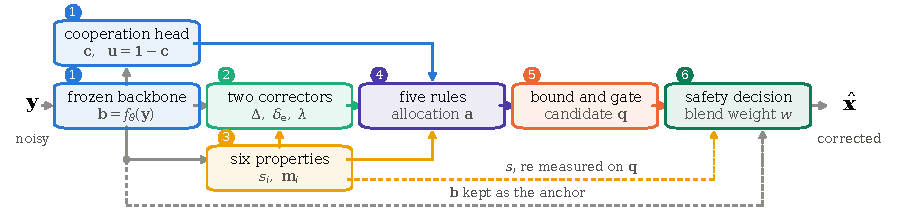
\includegraphics[width=\textwidth]{figures/architecture.pdf}
\caption{The six stages of the method. A frozen backbone produces the denoised image and a small head
estimates confidence. Two networks propose a multiplicative change and an additive edge change. Six
clinical properties are measured and produce a score and a failure map each. Five rules turn those
signals into a per pixel allocation. The admitted change is bounded, gated away from the background
and combined. Three constraints are then checked, and the number that pass decides how much of the
candidate replaces the backbone output.}
\label{fig:architecture}
\end{figure*}

\begin{table}[!tb]
\centering
\caption{Feature tensor read by the confidence head for each backbone. All heads share the same two
layer design and differ only in the number of input channels.}
\label{tab:uncertainty_sources}
\setlength{\tabcolsep}{4pt}
\footnotesize
\begin{tabular}{lll}
\toprule
Backbone & Feature tensor & Channels \\
\midrule
NAFNet & First encoder stage & 40 \\
KBNet & First encoder stage & 32 \\
DnCNN & First convolution & 228 \\
SwinIR & Shallow feature convolution & 138 \\
\bottomrule
\end{tabular}
\end{table}

\begin{table}[!tb]
\centering
\caption{The six clinical properties. Each one names a way a denoised OCT image is known to fail,
returns a score for the whole image and a map of where the property is unsatisfied, and is compared
against a threshold. The closed form of every score and every map is given in the supplementary file
and in the released code. Here $e$ is the Sobel edge magnitude of the backbone output, $\sigma_k$ is
the local standard deviation over a window of size $k$, and $cv$ is the local coefficient of
variation of the log residual.}
\label{tab:predicates}
\setlength{\tabcolsep}{3pt}
\footnotesize
\begin{tabular}{clp{0.40\columnwidth}c}
\toprule
$P_i$ & Property & Where the map is large & $\tau_i$ \\
\midrule
$P_1$ & edge continuity & away from detected edges, where a boundary should continue but does not & 0.60 \\
$P_2$ & local contrast & where $\sigma_9$ falls below the image mean, and in nearly flat tissue & 0.50 \\
$P_3$ & flat smoothness & inside flat regions that still carry residual variation & 0.75 \\
$P_4$ & structural coherence & where the edge map is itself rough, a sign of broken structure & 0.50 \\
$P_5$ & speckle conformity & where $cv$ departs from the value expected for OCT speckle & 0.30 \\
$P_6$ & layer visibility & where the local variance of the edge map is high across depth & 0.70 \\
\bottomrule
\end{tabular}
\end{table}

\begin{figure*}[!tb]
\centering
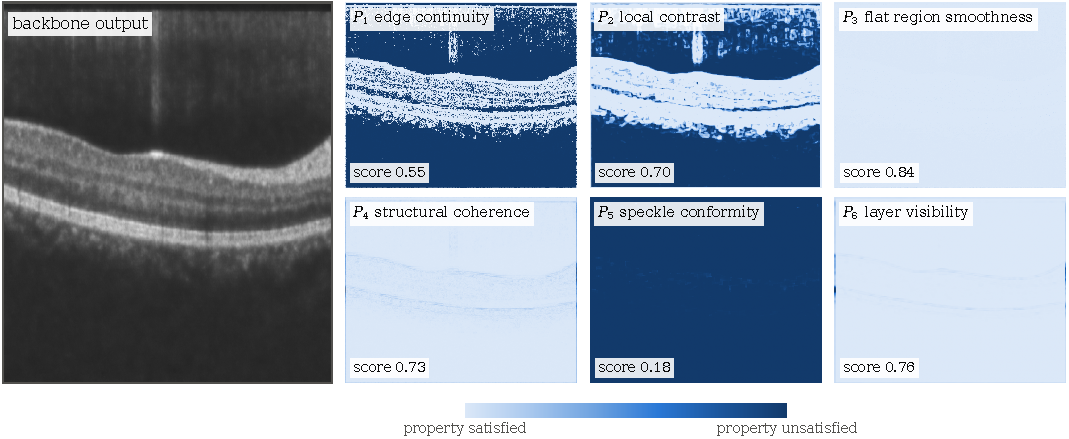
\includegraphics[width=0.98\textwidth]{figures/fig_predicate_maps.pdf}
\caption{The six clinical properties on one backbone output. Each panel shows where that property is
locally unsatisfied, on a shared scale, with the image level score in the corner. Edge continuity,
local contrast and speckle conformity carry most of the evidence on this image, while the other three
are close to satisfied everywhere.}
\label{fig:predicate_maps}
\end{figure*}

\section{Clinical Properties and Fuzzy Allocation}
\label{sec:properties_allocation}

\subsection{Stage three, the six clinical properties}
\label{sec:predicates}
Each of the six properties
names a way a denoised OCT image is known to fail and each is written as a formula so it can be
recomputed by anyone. Table~\ref{tab:predicates} gives, for every property, the reason it exists,
its score $s_i \in [0,1]$ as a weighted sum of named subterms, its map
$\mathbf{m}_i \in [0,1]^{H \times W}$ in closed form, where that map is large, and the threshold
$\tau_i$ that separates satisfied from unsatisfied, with every subterm defined beneath the table. A
larger score means the property is better satisfied and a larger map value means stronger local
evidence that it is not. None of these quantities needs a clean reference. They are computed from the
noisy input and the backbone output only, so they remain available at test time on a scanner the
method has never seen.

\subsection{Stage four, the rule layer}
\label{sec:negotiator}
The rule layer decides where the gain proposal should act through five named rules, each casting a
signed vote.

Each property score is first turned into a soft failure signal by comparing it with its threshold,
\begin{equation}
f_i = \sigma\big(\kappa (\tau_i - s_i)\big), \qquad \kappa = 10 ,
\label{eq:soft_failure}
\end{equation}
so $f_i$ is near one when property $i$ is failing and near zero when it is satisfied. The same soft comparison is used to test the cooperation
map and the strength of a proposal against their own thresholds. Each corrector produces that
strength as a per-pixel map from the backbone output and the failure maps it serves, large where its
property is far below threshold. Before the rules fire, that strength is multiplied by one half plus the
demand map, so the same proposal looks stronger to the rules at a pixel where the head reports low
cooperation. Conjunction uses the Lukasiewicz
form $\mathrm{AND}(a,b) = \max(0, a + b - 1)$, which is piecewise linear and has a bounded slope,
which is what makes the bound in Section~\ref{sec:stability} tight.

The five rules are the following. Rule one fires when the cooperation map is high and the proposal is
weak, and it votes against changing the image. Rule two fires when the map is low and the
proposal is strong, and it votes for changing it. Rule three fires when a relevant property is
failing, and it votes for changing it. Rule four fires when the map and the proposal strength are both
middling, and it votes weakly for changing it. Rule five fires when several correctors want the same
pixel, and it votes against changing it. Write $r_1$ to $r_5$ for the resulting truth values.

The allocation at each pixel is the bounded weighted vote
\begin{equation}
\begin{aligned}
a ={}& \underbrace{B_{\min} + (B_{\max} - B_{\min})\,\sigma(\beta)}_{\text{base, no rule firing}} \\
    &- C_1 w_1 r_1 + C_2 w_2 r_2 + C_3 w_3 r_3 + C_4 w_4 r_4 - C_5 w_5 r_5 ,
\end{aligned}
\label{eq:allocation}
\end{equation}
where $\beta$ is a learnable base logit, $w_k = \sigma(\theta_k) \in (0,1)$ are learnable rule weights
and the budgets are $B_{\min} = 0.25$, $B_{\max} = 0.50$, $C_1 = 0.15$, $C_2 = 0.25$, $C_3 = 0.15$,
$C_4 = 0.10$ and $C_5 = 0.10$.

The budgets satisfy $B_{\max} + C_2 + C_3 + C_4 = 1$ and
$B_{\min} - C_1 - C_5 = 0$, so since every truth value lies in $[0,1]$ and every weight in $(0,1)$,
the value of Equation~\eqref{eq:allocation} lies in $[0,1]$ for every input and every parameter value
and no clipping is ever needed. Without the identity a clamp is needed, the allocation saturates at
one end of it, as it did on every pixel in the submitted version of this work, the rule weights
receive no gradient, and the stability result of Section~\ref{sec:stability} is vacuous.
\label{sec:allocation_defect}

\section{Bounded Change and the Safety Decision}
\label{sec:bounded_safety}

\subsection{Stage five, applying the change}
\label{sec:composition}
The admitted gain is the raw proposal modulated by the allocation and the strength map, then bounded,
\begin{equation}
\boldsymbol{\alpha} = \mathrm{clamp}\big(\boldsymbol{\Delta} \odot \mathbf{a} \odot \boldsymbol{\lambda},\, -0.20,\, 0.20\big).
\label{eq:alpha}
\end{equation}
A gate suppresses any change in the dark background,
\begin{equation}
\mathbf{g} = \sigma\big(20\,(\mathbf{b} - q_{0.15})\big),
\label{eq:gate}
\end{equation}
where $q_{0.15}$ is the fifteenth percentile of the backbone output of that image. Using a percentile
rather than a fixed level makes the gate work across scanners with different brightness. A second form
of the gate, used where the selection of Section~\ref{sec:weight_selection} chose it, is a soft step at
the per image Otsu threshold followed by a maximum filter of fixed radius, so that the gate is
identically zero beyond that radius from tissue.

The gated gain is applied multiplicatively to give the change $\mathbf{v}$, with the brightening part
smoothed before it is added so that it cannot create a new high frequency edge,
\begin{equation}
\mathbf{v} = \big(\,\mathrm{smooth}(\mathrm{ReLU}(\boldsymbol{\alpha}) \odot \mathbf{b})
 + (\boldsymbol{\alpha} - \mathrm{ReLU}(\boldsymbol{\alpha})) \odot \mathbf{b}\,\big) \odot \mathbf{g},
\label{eq:apply}
\end{equation}
where $\mathrm{smooth}$ is a three by three mean filter. The darkening part is left unsmoothed because
it has zero mean and cancels itself. In the background, defined by the complement of the gate eroded
by two pixels, a masked three by three mean filter is blended in at half strength, which lowers the
background standard deviation without letting blur cross into tissue. Finally the edge proposal is
added and the result is clipped to the valid range,
\begin{equation}
\mathbf{q} = \mathrm{clamp}\big(\mathbf{b} + \mathbf{v} + \boldsymbol{\delta}_{\mathrm{e}} \odot \mathbf{g},\, 0,\, 1\big).
\label{eq:candidate}
\end{equation}

\subsection{Stage six, the safety decision}
\label{sec:safety}
The candidate $\mathbf{q}$ is not returned directly. Three constraints are checked on it.

\textbf{Aggregate quality must not fall.} Define for any image $\mathbf{t}$ the energy
\begin{equation}
E(\mathbf{t}) = 1 - \tfrac{1}{6}\sum_{i=1}^{6} s_i(\mathbf{t})
 + 0.1 \sum_{i=1}^{6} \max\big(0,\, 0.5 - s_i(\mathbf{t})\big),
\label{eq:energy}
\end{equation}
which is small when the image is good, and whose second term penalises any single property below one
half, so a good average cannot hide one broken property. The first constraint requires
$E(\mathbf{q}) \le E(\mathbf{b}) + 0.10$.

\textbf{No property may be sacrificed for another.} The second constraint requires that at least one
property improves by more than $0.01$ and that no property falls by more than $0.10$.

\textbf{The image must not move far.} The third constraint requires
$\lVert \mathbf{q} - \mathbf{b} \rVert_2 \,/\, \lVert \mathbf{b} \rVert_2 < 0.2$.

Let $n \in \{0,1,2,3\}$ be the number of constraints that hold. The output is
\begin{equation}
\hat{\mathbf{x}} = (1 - w)\,\mathbf{b} + w\,\mathbf{q},
\qquad
w = \begin{cases}
1, & n \ge 2, \\[2pt]
0.05 + 0.10\,\dfrac{n}{3}, & n < 2 .
\end{cases}
\label{eq:blend}
\end{equation}
Otherwise the output falls back to the backbone while retaining five to eight percent of the proposal,
so the decision remains visible rather than silently discarded.


\begin{figure*}[!tb]
\centering
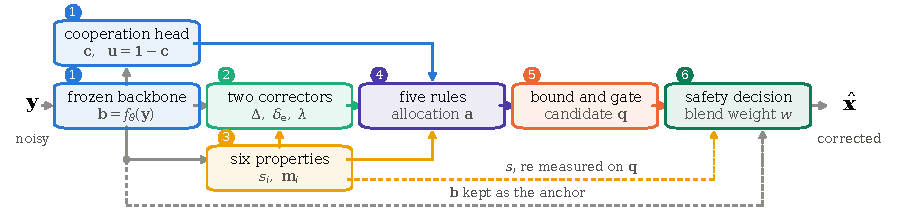
\includegraphics[width=0.783\textwidth]{figures/architecture.pdf}
\caption{The six stages. A frozen backbone and a small head produce the image and the cooperation
map. Two networks propose changes. Six properties are measured. Five rules allocate. The change is
bounded and gated. Three constraints decide how much is kept.}
\label{fig:architecture}
\end{figure*}


\begin{table*}[!tb]
\centering
\caption{The six clinical properties in closed form. Here $e$ is the Sobel edge magnitude of
$\mathbf{b}$, $\bar e$ its mean, $b_e = \mathbf{1}[e > \bar e]$, $\sigma_k$ and $\operatorname{Var}_k$
the local standard deviation and variance over a $k \times k$ window, $\bar\sigma$ the mean of
$\sigma_9$, $v(\cdot)$ the depth profile averaged across width, $\nabla_z$ the derivative along depth,
$\rho_h$ the one pixel horizontal autocorrelation, $\operatorname{sigm}$ the logistic function,
$\varepsilon$ a small constant, and $cv$ the local coefficient of variation of the log residual.}
\label{tab:predicates}
\setlength{\tabcolsep}{3pt}
\scriptsize
\begin{tabular}{clp{0.26\textwidth}p{0.225\textwidth}p{0.245\textwidth}c}
\toprule
$P_i$ & Property & Score $s_i$ & Map $\mathbf{m}_i$ & Where the map is large & $\tau_i$ \\
\midrule
$P_1$ & edge continuity &
$0.4\,c_{\text{cont}}+0.3\,c_{\text{efr}}+0.3\,c_{\text{ang}}$ &
$(1-\tilde e)(1-b_e)$, \ $\tilde e=e/(\max e+\varepsilon)$ &
off detected edges, where a boundary should continue but does not & 0.60 \\
$P_2$ & local contrast &
$0.20\,s_{\text{range}}+0.35\,s_{\text{cnr}}+0.20\,s_{\text{var}}+0.25\,s_{\text{cov}}$ &
$\big[\operatorname{ReLU}(\bar\sigma-\sigma_9(\mathbf{b}))/(\bar\sigma+\varepsilon)+0.3\,\mathbf{1}[\sigma_9(\mathbf{b})<0.01]\big]_{[0,1]}$ &
where $\sigma_9$ falls below the image mean, and in nearly flat tissue & 0.50 \\
$P_3$ & flat smoothness &
$0.6\,q_{\text{var}}+0.4\,q_{\text{res}}$ &
$F \odot \sigma_5(\mathbf{b})/(\max \sigma_5(\mathbf{b})+\varepsilon)$ &
inside flat regions that still carry residual variation & 0.75 \\
$P_4$ & structural coherence &
$0.4\,s_{\text{self}}+0.3\,s_{\text{reg}}+0.3\,s_{\text{vert}}$ &
$e(e)/(\max e(e)+\varepsilon)$ &
where the edge map is itself rough, a sign of broken structure & 0.50 \\
$P_5$ & speckle conformity &
$0.7\,\operatorname{mean}(\exp(-|cv-cv^\star|/0.15))+0.3\,\exp(-5|\rho_h(z)|)$ &
$1-\exp(-|cv-cv^\star|/0.15)$ &
where $cv$ departs from the value expected for OCT speckle & 0.30 \\
$P_6$ & layer visibility &
$0.4\,s_{\text{clr}}+0.3\,s_{\text{dep}}+0.3\,s_{\text{smo}}$ &
$\operatorname{Var}_7(e)/(\max \operatorname{Var}_7(e)+\varepsilon)$ &
where the local variance of the edge map is high across depth & 0.70 \\
\midrule
\multicolumn{6}{p{0.97\textwidth}}{
\textbf{Subterms.}
$P_1$.
$c_{\text{cont}}=\langle\operatorname{erode}(\operatorname{dilate}(b_e)),b_e\rangle/(\|b_e\|_1+\varepsilon)$,
$c_{\text{efr}}=\exp(-5|r_e-0.2|)$ with
$r_e=\|\mathbf{1}[e>1.5\bar e]\|_1/(\|\mathbf{1}[e<0.5\bar e]\|_1+\varepsilon)$,
and $c_{\text{ang}}=\exp(-2\,\operatorname{mean}(\sigma_5(\theta)))$ with $\theta$ the Sobel edge angle of $\mathbf{b}$.
$P_2$.
$s_{\text{range}}=\operatorname{sigm}(10(\Delta_r-0.3))$ with $\Delta_r=\max(\mathbf{b})-\min(\mathbf{b})$,
$s_{\text{cnr}}=\operatorname{sigm}(15(\bar\sigma-0.05))$,
$s_{\text{var}}=\max(0.2,\operatorname{sigm}(-20(v_\sigma-0.02)+2))$ with $v_\sigma=\operatorname{Var}(\sigma_9(\mathbf{b}))$,
and $s_{\text{cov}}=\operatorname{sigm}(5(\gamma-0.4))$ with $\gamma=\operatorname{mean}(\mathbf{1}[\sigma_9(\mathbf{b})>0.3\bar\sigma])$.
$P_3$.
$F=\mathbf{1}[e<0.3\bar e]$,
$q_{\text{var}}=1-\langle F,\sigma_5(\mathbf{b})/(\sigma_5(\mathbf{y})+\varepsilon)\rangle/(\|F\|_1+\varepsilon)$,
and $q_{\text{res}}=\exp(-5\,\operatorname{mean}|\mathbf{y}-\mathbf{b}|)$.
$P_4$.
$s_{\text{self}}$ is the mean Pearson correlation between $\mathbf{b}$ and its shifts by $(0,2)$, $(2,0)$ and $(2,2)$ pixels,
$s_{\text{reg}}=\exp(-12\,\operatorname{mean}(e(e)))$,
and $s_{\text{vert}}=\operatorname{clip}(\max |\nabla_z v(\mathbf{b})|/(8\,\operatorname{mean}|\nabla_z v(\mathbf{b})|),0,1)$.
$P_5$.
$z=\log(\mathbf{y}+\varepsilon)-\log(\mathbf{b}+\varepsilon)$,
$cv=\sigma_{15}(|z|)/(\mu_{15}(|z|)+\varepsilon)$ with $\mu_{15}$ the local mean,
and $cv^\star(d)$ is the target coefficient of variation of OCT speckle at axial depth $d$ under the Gamma K model of the released code.
$P_6$.
$s_{\text{clr}}=\operatorname{mean}(\operatorname{clip}(\max |\nabla_z v(\mathbf{b})|/(10\,\operatorname{mean}|\nabla_z v(\mathbf{b})|),0,1))$,
$s_{\text{dep}}=\operatorname{clip}(20\,\operatorname{Var}(v(\mathbf{b})),0,1)$,
and $s_{\text{smo}}=1-\operatorname{clip}(10\,\operatorname{mean}(\operatorname{Var}_z(\operatorname{mean}_w e)),0,1)$
with $\operatorname{mean}_w$ the mean across width and $\operatorname{Var}_z$ the variance along depth.} \\
\bottomrule
\end{tabular}
\end{table*}

\section{Stability and Guarantees}
\label{sec:stability}

This section defines the notion of stability that is used, proves that the rule layer has it, and
gives the condition under which the correction cannot reduce contrast. Section~\ref{sec:theory_check}
tests both results on real images.

\subsection{What stability means here}
\label{sec:stability_def}
This is not stability in the sense of Lyapunov and we claim no fixed point. The quantity that must
not behave erratically is the decision of the rule layer, a function of the five rule truth values,
which are exactly what shift when the backbone or the scanner changes.

\begin{definition}[Stability of the allocation]
\label{def:stability}
Let $\mathbf{r} = (r_1, \ldots, r_5) \in [0,1]^5$ be the vector of rule truth values at one pixel and
let $a(\mathbf{r})$ be the allocation of Equation~\eqref{eq:allocation} at that pixel with the
parameters held fixed. The allocation is said to be stable with constant $L$ if
\begin{equation}
\big| a(\mathbf{r}) - a(\mathbf{r}') \big| \;\le\; L \, \lVert \mathbf{r} - \mathbf{r}' \rVert_\infty
\qquad \text{for all } \mathbf{r}, \mathbf{r}' \in [0,1]^5 .
\label{eq:stability_def}
\end{equation}
\end{definition}

In words, a small change in the evidence produces a proportionally small change in the decision, and
$L$ is the worst case ratio between the two. Without such a bound the layer could swing from applying
no correction to applying all of it because one property score moved slightly, which is precisely
the behaviour a clinical user cannot audit.

\subsection{The rule layer is stable, with an exact constant}

\begin{theorem}[Allocation stability]
\label{thm:stability}
The allocation of Equation~\eqref{eq:allocation} satisfies Definition~\ref{def:stability} with
\begin{equation}
L \;=\; C_1 w_1 + C_2 w_2 + C_3 w_3 + C_4 w_4 + C_5 w_5 ,
\label{eq:lipschitz}
\end{equation}
where $w_k = \sigma(\theta_k)$ are the learned rule weights. The constant is attained, so it is the
exact Lipschitz constant and not merely an upper bound. Moreover $L < C_1 + C_2 + C_3 + C_4 + C_5 =
0.75$ for every possible setting of the parameters.
\end{theorem}

The allocation is affine in $\mathbf{r}$ with coefficients $\pm C_k w_k$, so the bound follows from
the triangle inequality and is attained when each $r_k - r'_k$ takes the sign of its coefficient. The
full proof is given in the supplementary file.

\begin{corollary}[Behaviour under a change of backbone]
\label{cor:transfer}
Suppose replacing one backbone by another changes the rule truth values at a pixel by at most
$\epsilon$ in the maximum norm, with the parameters unchanged. Then the allocation at that pixel
changes by at most $L\epsilon$, with $L$ from Equation~\eqref{eq:lipschitz}.
\end{corollary}

This is a statement about the routing rule alone. It says the decision layer degrades gracefully when
the evidence shifts, not that image quality transfers, which is the empirical question of
Section~\ref{sec:results_ood}.

\subsection{When the correction cannot reduce contrast}
Contrast to noise ratio is the measure this method targets most directly. Write
$\mathrm{CNR}(\mathbf{t}) = (\mu_\mathcal{T}(\mathbf{t}) - \mu_\mathcal{B}(\mathbf{t})) / \sigma_\mathcal{B}(\mathbf{t})$
for the separation between tissue and background divided by the variability of the background.

\begin{theorem}[Contrast margin]
\label{thm:cnr}
Let $\eta_\mathcal{T} = \mu_\mathcal{T}(\mathbf{q}) - \mu_\mathcal{T}(\mathbf{b}) \ge 0$ be the gain in
tissue mean and let $\eta_\mathcal{B} \ge \mu_\mathcal{B}(\mathbf{q}) - \mu_\mathcal{B}(\mathbf{b})$
bound the leakage into the background. If the correction does not raise the background variability,
that is $\sigma_\mathcal{B}(\mathbf{q}) \le \sigma_\mathcal{B}(\mathbf{b})$, then the output of
Equation~\eqref{eq:blend} satisfies
\begin{equation}
\mathrm{CNR}(\hat{\mathbf{x}}) \;\ge\;
\frac{\big(\mu_\mathcal{T}(\mathbf{b}) - \mu_\mathcal{B}(\mathbf{b})\big) + w\,(\eta_\mathcal{T} - \eta_\mathcal{B})}
     {\sigma_\mathcal{B}(\mathbf{b})} .
\label{eq:cnr_bound}
\end{equation}
In particular, whenever $\eta_\mathcal{T} > \eta_\mathcal{B}$ the correction cannot reduce the
contrast to noise ratio.
\end{theorem}

\noindent The proof is a convex combination argument for the numerator and Minkowski's
inequality for the denominator. It is given in full in the supplementary file.


Three parts of the design make the hypotheses of Theorem~\ref{thm:cnr} hold in practice. The gate of
Equation~\eqref{eq:gate} keeps $\eta_\mathcal{B}$ small by suppressing change in the dark region, the
brightness branch of the gain network cannot be negative, which keeps $\eta_\mathcal{T}$ non negative,
and the background smoothing lowers $\sigma_\mathcal{B}(\mathbf{q})$ rather than raising it.
Section~\ref{sec:theory_check} measures all three on every test image and reports how often the
hypotheses hold.

Both results are deliberately narrow. Theorem~\ref{thm:stability} bounds how far the routing decision
can move, not whether it is correct, Theorem~\ref{thm:cnr} concerns contrast alone and says nothing
about the other five measures, and neither promises that the output is closer to the clean reference,
which Section~\ref{sec:results_id} shows it usually is not. The guarantees concern the policy, not the
denoiser underneath it.

\section{Training}
\label{sec:training}

\subsection{The five loss terms}
\label{sec:loss_terms}
Let $\mathbf{x}$ be the clean reference, $\mathbf{b}$ the backbone output and $\hat{\mathbf{x}}$ the
wrapper output. The objective of Equation~\eqref{eq:objective} has the following terms.

\textbf{Fidelity.} This term combines the squared error with
the structural similarity index~\cite{wang2004image},
\begin{equation}
\mathcal{L}_{\mathrm{fid}} = \lVert \hat{\mathbf{x}} - \mathbf{x} \rVert_2^2
 + \big(1 - \mathrm{SSIM}(\hat{\mathbf{x}}, \mathbf{x})\big).
\label{eq:loss_fid}
\end{equation}
A dead zone is applied to the peak signal to noise ratio part of this term, so no penalty is charged
while the drop with respect to the backbone stays below $d$ decibels.

\textbf{Clinical improvement.} This term rewards a rise in the clinical measures relative to the
backbone, beginning with the contrast to noise ratio and the tissue contrast index, TCI. The logarithm
of a ratio makes the term scale free,
\begin{equation}
\mathcal{L}_{\mathrm{clin}} = -\log\frac{\mathrm{CNR}(\hat{\mathbf{x}})}{\mathrm{CNR}(\mathbf{b})}
 - \log\frac{\mathrm{TCI}(\hat{\mathbf{x}})}{\mathrm{TCI}(\mathbf{b})}.
\label{eq:loss_clin}
\end{equation}
The same construction is added for the edge preservation index, the equivalent number of looks and
the signal to noise ratio, each with its own weight, so a gain in one measure cannot be bought by a
collapse in another.

\textbf{Property calibration.} The rule layer compares each property score with a threshold, and if the scores drift away from the
thresholds the comparison becomes uninformative, so this term pulls the scores toward the operating
point,
\begin{equation}
\mathcal{L}_{\mathrm{pred}} = \sum_{i=1}^{6}\big(s_i(\hat{\mathbf{x}}) - \tau_i\big)^2 .
\label{eq:loss_pred}
\end{equation}

\textbf{Cooperation.} The wrapper should act where the backbone is unsure and stay quiet where it is
confident. We measure the agreement between the demand map $\mathbf{u}$ and $\boldsymbol{\pi}$, the summed
strength map of the two proposals that the rule layer of Section~\ref{sec:negotiator} reads, with the
Pearson correlation $\rho$, and penalise disagreement,
\begin{equation}
\mathcal{L}_{\mathrm{coop}} = \tfrac{1}{2}\,\mathrm{ReLU}\big(1 - \rho(\mathbf{u}, \boldsymbol{\pi})\big).
\label{eq:loss_coop}
\end{equation}
The Pearson correlation is differentiable everywhere, invariant to an affine change of either map, and
introduces no window size to tune.

\textbf{Edge supervision.} The additive branch is trained to reproduce the gradient that the backbone
lost, measured with the Sobel operator $\nabla$,
\begin{equation}
\mathcal{L}_{\mathrm{edge}} = \big\lVert \nabla\hat{\mathbf{x}} - \nabla\mathbf{x} \big\rVert_2^2 .
\label{eq:loss_edge}
\end{equation}

\subsection{Data and optimisation schedule}
\label{sec:paired_data}
Training uses paired data, a noisy scan and a clean reference averaged over repeated acquisitions,
and the reference enters the fidelity and clinical terms and supervises the edge branch. Testing uses
no clean image at any point, since the six properties read only the noisy input and the backbone
output, and the reference only scores the results. The backbone is trained first, on the training split with the squared error alone, and is then
frozen. The wrapper is then trained in two stages. Only the clinical terms are active at first, so
the correctors learn a useful direction, and the fidelity term switches on at the midpoint, so they
learn how far they may go. Both stages use AdamW with weight decay $10^{-4}$ on $96 \times 96$ crops
in batches of sixteen, eight for DnCNN and SwinIR, for ten epochs in all, with base learning rates of
$2 \times 10^{-4}$ for the corrector networks, $5 \times 10^{-4}$ for the cooperation head and the
strength predictor and $3 \times 10^{-4}$ for the rule layer, and the output layers of the correctors
and the background smoother at two to eight times the corrector rate. The supplementary file restates
the procedure as pseudocode.

Throughout both stages the normalisation statistics of $f$ are held fixed. DnCNN is the one backbone with batch normalisation, and left in training mode 45 of its
buffers move during fitting, so the frozen reference against which every clinical change of that
backbone is measured reads 30.68 dB and a boundary sharpness of 1.031 when the statistics are held
fixed against 31.21 dB and 0.948 when they are not.

\subsection{How the operating point was chosen}
\label{sec:weight_selection}
The terms of Equation~\eqref{eq:objective} carry fixed relative weights. The training script can
also learn them through an uncertainty weighting, and that path is inactive in every run reported
here, which the absence of its parameters from the released checkpoints confirms. Two quantities are selected
per backbone on the validation split, the fidelity dead zone $d$ of Equation~\eqref{eq:loss_fid} and
the rule of Equation~\eqref{eq:gate} that decides where a correction may act. The grid is the two
gate rules crossed with dead zones of 0.3, 0.6 and 0.9 dB, and the tissue bounded gate crossed with
radii of 41 and 61 pixels. It selected the tissue bounded gate at radius 41 and a dead zone of 0.6 dB
for NAFNet, and the percentile gate at a dead zone of 0.9 dB for the other three. Everything else is
held at one value for every backbone and every run. For each backbone every setting is trained at three random seeds
and scored on the validation images. A setting is admissible only if it clears its bounds at its
\emph{worst} seed rather than on average, and among the
admissible settings we take the one with the largest lower confidence bound on its weakest clinical
measure. When no setting clears the first pair of bounds we relax them one step at a time and record
the step that was needed, so a backbone that required a looser condition is visible rather than
hidden. Every source of randomness is seeded, up to the nondeterminism of the convolution kernels, and
the checkpoints chosen on validation are the checkpoints scored on test.

\subsection{Initialisation and the choice of every constant}
\label{sec:constants}
Every constant appears with its value where it acts and has one of four origins. Fixed structural
choices, never tuned, are the sharpness $\kappa = 10$ of
Equation~\eqref{eq:soft_failure}, the steepness 20 of Equation~\eqref{eq:gate}, the window sizes, the
quarter resolution of the gain network, the nominal bound $\pm 0.08$ of the edge branch, the
thresholds $\tau_i$ of Table~\ref{tab:predicates}, taken from the clinical literature and unchanged by
training to four decimals in every run, and the budgets
$B$ and $C$, tied by the identity of Section~\ref{sec:allocation_defect}. Set once on the validation
split while the method was built and never revisited are $\alpha_{\max} = 0.15$, the gain bound
$\pm 0.20$, the gate percentile 0.15, the three tolerances of Section~\ref{sec:safety}, the half
strength background blend and the learning rates. Selected in the grid of
Section~\ref{sec:weight_selection}, on the validation split only, are the dead zone $d$ and the gate
rule. Learned by the objective are $\beta$, $\theta_1$ to $\theta_5$, $\tau_0$, $\beta_0$ and the
scale of the edge branch. Every layer uses its default initialisation with one deliberate exception,
the bias of the brightness channel of the gain network starts at 0.5, so the raw gain begins at
$0.5\,\alpha_{\max}$ in flat tissue rather than on a flat region of the loss. Nothing was ever chosen
on the test split, and Section~\ref{sec:sensitivity} reports how much the results move when the
constants of the rule layer are changed, the direct test of whether any of them does hidden work.



\section{Tests and Results}
\label{sec:tests}

\subsection{Setup}
\label{sec:setup}

\emph{Data.} PKU37~\cite{geng2022triplet} provides 37 cross sections of $640 \times 640$ pixels from a
spectral domain scanner, references averaged over 50 frames, split by clean image identity into 27, 5
and 5 for training, validation and testing, giving 1388, 173 and 173 pairs, and is the only training
domain. Duke17~\cite{fang2012sparsity} provides 17 paired B scans of $970 \times 520$ from a clinical
scanner at another institution, of which we use the 16 stored under the naming the released loader
reads, and Duke2013~\cite{fang2013fast} the 18 volumes of $900 \times 450$ of its test split.

\emph{Transfer protocol.} Every model is trained once on PKU37 and applied to the Duke sets directly,
with nothing fitted, recalibrated or selected on Duke data beyond the per image quantity the gate of
Equation~\eqref{eq:gate} computes by the same rule as on PKU37. The original submission instead
adapted the wrapper for fifteen further epochs on the other subjects of the target set, leave one
subject out, backbone frozen, with an L2 penalty holding every trainable weight near its PKU37 value,
and we rerun that for NAFNet in the adapted block of Table~\ref{tab:pku37}, with per subject spreads
in the supplementary file.

\emph{Measures.} Peak signal to noise ratio against the clean reference measures fidelity. Six
clinical measures, given as percentage change from backbone to corrected output, are contrast to
noise ratio for tissue against background, tissue contrast index for dynamic range in tissue, edge
preservation index for agreement with the reference edge map, boundary sharpness for the gradient
across layer boundaries, equivalent number of looks for speckle suppression, and signal to noise
ratio against the noise floor. Each is computed per image then averaged, never pooled across a batch,
since pooling inflates the result. 

\begin{table*}[!tb]
\centering
\caption{PKU37 test set of 173 images, then Duke17 and Duke2013 with no adaptation, then the adapted
protocol of the original submission for NAFNet described in Section~\ref{sec:setup}. Columns give the
backbone peak signal to noise ratio in decibels, its change after correction with the spread across
three seeds, and the six clinical measures as percentage change from backbone output to corrected
output, bold where the mean exceeds the seed spread. The adapted rows come from one seed and one fold
per subject, so they carry no spread and no bold. The two lowest blocks use the selected NAFNet checkpoint on the
same 173 test images with one component removed or an alternative operator substituted. Full spreads
are in the supplementary file.}
\label{tab:pku37}
\setlength{\tabcolsep}{4pt}
\footnotesize
\begin{tabular}{lccccccc}
\toprule
Backbone & $\Delta$PSNR & $\Delta$CNR & $\Delta$TCI & $\Delta$EPI & $\Delta$BS & $\Delta$ENL & $\Delta$SNR \\
\midrule
NAFNet & -0.18 & $\mathbf{+3.49}$ & $\mathbf{+1.91}$ & $\mathbf{+1.20}$ & $\mathbf{+3.89}$ & $\mathbf{+23.74}$ & $\mathbf{+11.10}$ \\
DnCNN & -0.98 & $\mathbf{+11.30}$ & +0.99 & $\mathbf{+4.14}$ & -1.44 & $\mathbf{+57.14}$ & $\mathbf{+22.95}$ \\
SwinIR & -0.17 & $\mathbf{+7.33}$ & $\mathbf{+11.45}$ & $\mathbf{+2.68}$ & $\mathbf{+1.82}$ & $\mathbf{+28.32}$ & $\mathbf{+11.54}$ \\
KBNet & -0.90 & $\mathbf{+6.93}$ & $\mathbf{+5.92}$ & +0.00 & $\mathbf{+2.58}$ & $\mathbf{+25.30}$ & $\mathbf{+7.95}$ \\
\bottomrule
\end{tabular}

\end{table*}

\subsection{In distribution results}
\label{sec:results_id}
Table~\ref{tab:pku37} reports the PKU37 test set and Fig.~\ref{fig:subjective_pku37} the visual
comparison across the four backbones. Contrast rose on 2064 of the 2076 image and seed combinations.
The twelve exceptions all belong to NAFNet, the backbone with the smallest mean contrast gain, fall on
ten images whose backbone PSNR lies above the NAFNet mean, and none exceeds 0.4 percent. The gain was
larger where the backbone PSNR was lower, with a per image Spearman correlation between minus 0.46 and
minus 0.71 across the four backbones. Of the 24 backbone by measure pairs, 21 are positive by more
than one seed spread, one is positive but inside it, the tissue contrast index of DnCNN, one is
unchanged at 0.00 percent, the edge preservation of KBNet, and one falls, the boundary sharpness of
DnCNN at minus 1.44 percent. The fidelity cost ranges from 0.17 dB on SwinIR to 0.98 dB on DnCNN, and
the two backbones that pay least are the two whose six measures all rise.

\begin{figure*}[!tb]
\centering
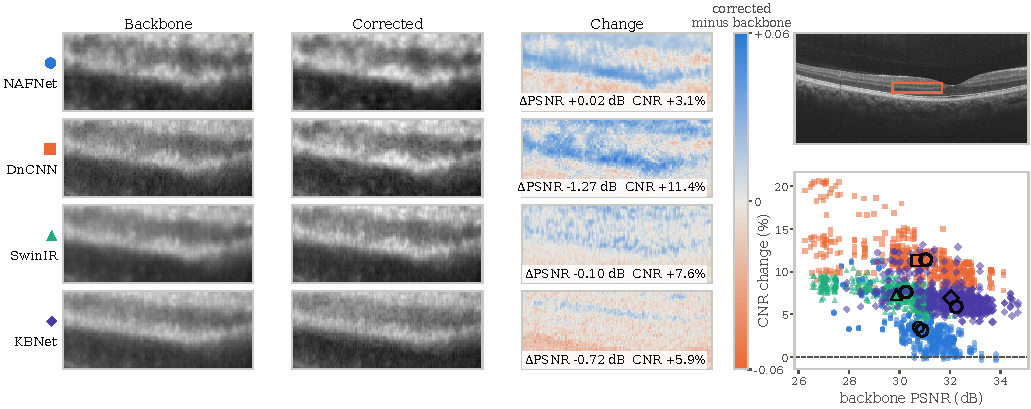
\includegraphics[width=0.9\textwidth]{figures/fig_subjective_pku37.pdf}
\caption{Visual comparison on the PKU37 test image of median backbone fidelity, one row per backbone,
in the 56 by 136 pixel band marked on the thumbnail where the NAFNet correction was largest. The
eight gray cells share one display range, set to the values they contain so that nothing is clipped,
and the signed difference uses a fixed scale of plus or minus 0.06. The mean absolute change is about
one percent of the intensity range, most for SwinIR and least for KBNet, from the seed 0 checkpoints
of Table~\ref{tab:pku37}. The scatter places this image, ringed, among all 173 test images at three
seeds for four backbones, with the twelve NAFNet points below zero marked. Full resolution pairs for
every backbone are in the supplementary file.}
\label{fig:subjective_pku37}
\end{figure*}

\subsection{Transfer to other scanners}
\label{sec:results_ood}
Table~\ref{tab:pku37} reports the no adaptation protocol on Duke17 and Duke2013. All six clinical
measures are positive on both target sets for NAFNet and SwinIR, the fidelity cost stays inside
0.35 dB for those two, and 40 of the 48 backbone by measure by set pairs are positive, the eight
exceptions being the tissue contrast index and the boundary sharpness of DnCNN and the edge
preservation and the signal to noise ratio of KBNet. Contrast rises on every backbone and both sets.

Adaptation, the last block, raises contrast on both scanners, from $+7.5$ to $+10.7$ percent on
Duke17 and from $+7.4$ to $+15.4$ on Duke2013, where it also lifts the tissue contrast index from
$+1.4$ to $+5.1$. It pays on both, a further 0.06 and 0.10 dB of fidelity and a signal to noise ratio
that falls from $+5.4$ to $+2.9$ percent on Duke17 and from $+9.3$ to $-5.3$ on Duke2013, down on 15
of 18 subjects, while the other measures move in opposite directions on the two sets. The only
measure adaptation reliably improves is the one the frozen model already improves, so the frozen
model is the one we recommend and use everywhere else.

\subsection{Contribution of each clinical property}
\label{sec:predicate_ablation}
One property at a time is switched off
at test time, by setting its score to the satisfied value and its failure map to zero, and the whole
test set is re evaluated. Only $P_5$, $P_1$ and $P_2$ move any measure by more than a quarter point.
$P_5$ costs the most at 3.19 points of the speckle gain, $P_1$ 1.72 and $P_2$ 0.74, while $P_3$,
$P_4$ and $P_6$ change nothing by more than 0.23 points. We keep all six, because they are the vocabulary of the rule layer and of the explanation shown to the
reader, and one that rarely fires here can fire on another scanner.

\subsection{Sensitivity to the rule constants}
\label{sec:sensitivity}
The rule layer contains a base level, five rule weights and five budgets. The budgets are tied by the identity of Section~\ref{sec:allocation_defect}, so they are held. We
vary the base level and the two
rule weights that carry the allocation, and we replace the Lukasiewicz conjunction by the product and
by the minimum, the two other standard choices, to test whether the specific logic matters. No
variation turns any of the six clinical measures negative. Across the fourteen variations the
contrast gain lies between 3.5 and 4.5 percent, the tissue contrast index between 2.3 and 2.9
percent, the speckle measure between 22.6 and 23.5 percent and the fidelity cost between 0.16 and
0.23 dB. The base level is the only constant whose effect is visible, since lowering it raises
contrast and costs fidelity together, while the two rule weights move the result by under a fifth of
a point. The product and the minimum change the contrast gain from 3.7 to 3.5 percent and leave the
other five measures within one part in fifty, so the result rests on the shape of the rule layer and
not on the particular conjunction. No setting of either gate rule of
Section~\ref{sec:weight_selection} recovers boundary sharpness on DnCNN.

\subsection{Contribution of each component}
\label{sec:component_ablation}
The component block of Table~\ref{tab:pku37} removes one component at a time. Replacing the rule layer by a uniform
allocation cuts the contrast gain from 3.7 to 0.8 percent and the tissue contrast index from 2.4 to
0.4 percent while doubling the fidelity cost, the clearest evidence that the allocation and not the
capacity of the correctors produces the clinical gain. Removing the edge branch turns both measures
negative, and removing the cooperation map costs about a third of the contrast gain. Removing
background smoothing leaves contrast, edge preservation and boundary sharpness almost intact while
the speckle measure collapses from 23.3 to 5.8 percent and the signal to noise ratio from 10.7 to 2.9
percent.

\subsection{Comparison at matched complexity}
\label{sec:matched}
Three alternatives act on the same frozen backbone output. The first is the same architecture, budget,
objective and ten epochs, with the rule layer replaced by a uniform allocation for the whole of
training rather than only at test time, keeping the properties and the safety layer. It was fitted
before the gate search, so it carries the percentile gate rather than the tissue bounded gate NAFNet
was finally selected with. The other two are classical operators, unsharp masking and contrast limited
adaptive histogram equalisation, tuned on the validation split. Uniform allocation reaches a larger
contrast gain and a much larger tissue contrast index than the full method, for 0.42 dB against 0.17
dB, and is worse on four of the six measures, so the two are not ordered. What the full method buys
with its fidelity is the per pixel account of why each change was made. The classical operators give
the largest contrast numbers and fail elsewhere, lowering edge preservation by about 3.5 percent and
the speckle measure by about 36 percent while raising boundary sharpness by about 25 percent by
sharpening noise with structure, with adaptive equalisation also costing 4.4 dB.


\subsection{Does the cooperation map predict error}
\label{sec:confidence_check}
Called a confidence map in the original submission, this component was tested against the absolute
error of the backbone output over \NImages{} images, and it does not predict that error. The rank
correlation is \CalibRho{}, so the map is ordered the wrong way rather than merely uninformative, and
removing the pixels it ranks as least reliable raises the remaining error to 1.88 times the starting
value where an oracle ranking reaches 0.07, a sparsification error of \CalibAuse{}. The map is
nevertheless load bearing, since replacing it by a constant lowers the contrast gain from $+3.71$ to
$+2.51$ percent and worsens five of the six clinical measures. Nothing in the objective shows the head the error of the backbone, so we call it a cooperation map
rather than a confidence.

\subsection{Do the theoretical conditions hold on real data}
\label{sec:theory_check}
We perturb the rule truth values and compare the ratio of Equation~\eqref{eq:stability_def} with the
constant of Equation~\eqref{eq:lipschitz}, and we measure the tissue gain, the background leakage and
the ratio of background standard deviations on every image against the hypotheses of
Theorem~\ref{thm:cnr}. The stability bound holds with room to spare, a constant of \LipTheory{} from
Equation~\eqref{eq:lipschitz} against a largest measured ratio of \LipMeasured{} over \NImages{}
images, so the proof is conservative rather than tight. The
allocation map spans \AllocMin{} to \AllocMax{} with mean \AllocMean{} and standard deviation
\AllocStd{}, and \AllocClamp{} percent of pixels sit at either end of its clamp, direct evidence that
the rule layer does work after the repair of Section~\ref{sec:allocation_defect}.

The margin condition holds on
\CondMargin{} of \NImages{} images and the standard deviation ratio condition on \CondSigma{}, a bare
majority, with mean ratio \SigmaRatio{} below one, which is why the result holds in the mean. Where a
hypothesis fails the theorem predicts nothing, and the measured contrast change there does not differ
systematically in sign, so the conditions are sufficient and not necessary. Both leakage terms of
Theorem~\ref{thm:cnr} sit far below the mean absolute change over the whole image, \GlobalChange{}, at
\EtaT{} in tissue and \EtaB{} in background, with means near zero and a long negative tail, so the per
image sign carries what the theorem needs. Tissue is positive on \EtaTPos{} of \NImages{} images and
background negative on \EtaBNeg{}, the direction the decomposition assumes.

\subsection{Safety, and whether the correction invents structure}
\label{sec:safety_check}
A correction that raises contrast could sharpen a boundary that is not there or erase a faint one
that is, and the clean reference lets us measure both. Two measures move against it. An edge appears where the
reference has none on \EdgeInvCorr{} percent of pixels after correction against \EdgeInvBack{} percent
for the backbone output, a rise on \EdgeInvUp{} of \NImages{} images with $p = 1.9 \times 10^{-12}$ under a two
sided Wilcoxon signed rank test on the paired per image values, and the retention of structures whose
reference contrast falls in the lowest decile falls from \WeakRetBack{} to \WeakRetCorr{} percent, on
\WeakRetDown{} of \NImages{} images with $p = 6.2 \times 10^{-30}$. Both are small, 0.03 points of invented
edge rate and 2.9 points of retention, neither is zero by construction, since the clamp of
Section~\ref{sec:safety} bounds how far a pixel may move and not how many cross an edge threshold, and
Section~\ref{sec:discussion} lists both as limitations. What separates the correction from a
sharpening filter is Section~\ref{sec:matched}, where the classical sharpeners lose edge preservation
and the speckle measure while the wrapper gains on both. The two
layer boundaries a clinician reads are not displaced, with a mean absolute shift of \IlmShiftBack{} to
\IlmShiftCorr{} pixels for the inner limiting membrane, an improvement, and \RpeShiftBack{} to
\RpeShiftCorr{} for the retinal pigment epithelium, unchanged within the spread across images. Dark
fluid like regions occupy \DarkFrac{} percent of the image area with a mean absolute change of
\DarkChange{} inside them against \GlobalChange{} over the whole image, and the largest change on any
single image anywhere in the test set is \GlobalMax{}, so the correction is quieter
where a dark region carries the finding. Boundary sharpness is not worsened on \BoundOK{} of
\NImages{} images, a count, since the per image worst case is what matters for trusting a scan. Of the three constraints of
Section~\ref{sec:safety}, energy holds on \ConEnergy{} of \NImages{} images and bounded change on
\ConLip{}, and only the no sacrifice constraint ever fails, on \NImages{} minus \ConPareto{} of them. Acceptance needs two of three and no image falls
below two, so the blend of Equation~\eqref{eq:blend} returns the candidate in full everywhere and the
safety layer never had to act here.

\subsection{Cost of moving to a new backbone}
\label{sec:transfer_cost}
A new backbone means refitting the whole wrapper, not only the head that reads its features. The
trainable count is \num{168630} shared parameters plus a head whose width follows the feature tensor it
reads, \num{175893} in all for NAFNet and \num{254538} for SwinIR, against about seven million in the
backbone, an increase of about 2.4 percent.
Every backbone is fitted on the same 1388 PKU37 pairs for the same ten epochs, so only the wall clock
time and the spread across seeds vary. Fitting one seed of the selected setting on a single RTX 5070
Ti takes 2.0 minutes for NAFNet, 2.5 for KBNet, 3.9 for DnCNN and 8.3 for SwinIR, an ordering that
follows the cost of one backbone forward pass. The spread of the
fidelity cost across the three seeds is 0.02 dB for NAFNet, 0.06 for SwinIR, 0.08 for KBNet and 0.21
for DnCNN. The backbone with the widest spread is also the only one with a clinical measure that
falls, so a new user should read the seed spread as the first warning sign rather than the mean.















\section{Discussion}
\label{sec:discussion}

\subsection{Why fidelity falls, and when that is the right trade}
\label{sec:psnr_tradeoff}
Peak signal to noise ratio usually falls slightly when the wrapper is applied, and the size of the
drop differs by backbone. This is not an accident of tuning. It follows from what the two objectives
reward. A denoiser trained on squared error is at a local optimum of that error, so any change to its
output moves away from that optimum. The wrapper makes changes that raise contrast and boundary
definition, and those changes are not free in squared error terms. The question is therefore not how
to avoid the drop but how to decide when it is worth accepting.

Two things decide it. A change of a few tenths of a decibel is smaller than the variation between two
acquisitions of the same eye, so it does not change what a downstream algorithm can do. And the
quantities that improve, namely boundary definition and tissue to background separation, are what a
grader actually uses to place a segmentation boundary or judge a fluid pocket.

The backbone that loses most fidelity is the one that had suppressed the most contrast to begin with.
A transformer with windowed attention smooths aggressively inside a window, which is efficient for
squared error and costly for local contrast. The wrapper restores that contrast, and restoring it
necessarily moves the pixels further from the smoothed optimum. The pattern is therefore informative
rather than embarrassing. The size of the correction tracks how much the backbone had given away.

For a deployment that must not lose fidelity at all, the safety layer already provides the control.
Tightening the third constraint of Section~\ref{sec:safety} reduces the admitted change, and the
result moves smoothly toward the backbone output. What the method does not offer is a free lunch in
which every measure improves at once, and we prefer to say so.

\subsection{What the formal results buy, and what they do not}
Theorem~\ref{thm:stability} is exact and it is about the code that ran. The constant follows from the
trained weights and Section~\ref{sec:theory_check} measures the realised ratio against it. That is a
different claim from a bound that holds vacuously because a clip enforces it.

Theorem~\ref{thm:cnr} is a sufficient condition rather than a guarantee of improvement. It says which
three quantities have to behave for contrast not to fall, and the method is built to make all three
behave. Reporting how often they actually hold, rather than asserting that they must, is the honest
form of that claim.

\subsection{Why the correction layer is worth its complexity}
A plain network with the same parameter budget can also improve clinical measures, as
Section~\ref{sec:matched} shows. What it cannot do is say why it changed a pixel. Every change made
here can be traced to a named property, a location where that property was measured to fail, a rule
that fired, and a safety decision that admitted the result. That trace is the product, and the
comparison at matched complexity is what shows the trace is not bought by giving up performance.

\subsection{Limitations}
The correction is bounded by construction, so a backbone that has destroyed a structure cannot be
made to recover it. The formal results are narrow in the way stated at the end of
Section~\ref{sec:stability}. The confidence head is the one part that must be refitted for a new
backbone, and Section~\ref{sec:transfer_cost} reports what that costs rather than treating it as
free. The clinical measures used here are established proxies, not outcomes, and no clinician read
the images, so the safety analysis of Section~\ref{sec:safety_check} is quantitative evidence rather
than clinical validation. Finally, the external datasets are small, sixteen and eighteen images, so
the transfer results should be read as evidence of behaviour across scanners rather than as a
precise estimate of the gain on any one device.

\section{Conclusion}
\label{sec:conclusion}

We presented a post-correction layer for OCT denoising, attached to a frozen denoiser rather than
replacing it. It states six clinical properties in closed form, turns them into a per-pixel decision through five
named rules, and limits how far the change may move the image, so any change traces back to the
property that motivated it. Across four backbone families the same rules, budgets and loss weights raise the clinical
measures at a fidelity cost below one decibel, and on three of the four no measure falls at all. The
exception is boundary sharpness on DnCNN, which starts above the clean reference, where the method has
no room to act. The measures are proxies, and the next step is a reader study.


% The class sets the bibliography at 8 pt through \bibliofont. A third of a point
% smaller keeps the last entries on the page they belong to, and the journal sets
% references below body size in any case.
\makeatletter
\def\bibliofont{\fontfamily{\rmdefault}\fontsize{7.5}{8.5}\selectfont}
\makeatother
\begin{thebibliography}{26}
\setlength{\itemsep}{0pt}
\setlength{\parsep}{0pt}

\bibitem{huang1991optical}
D.~Huang \emph{et al.}, ``Optical coherence tomography,'' \emph{Science}, vol.~254, no.~5035, pp.~1178--1181, 1991.

\bibitem{goodman2007speckle}
J.~W.~Goodman, \emph{Speckle Phenomena in Optics: Theory and Applications}.\hskip 1em plus 0.5em minus 0.4em Roberts \& Company, 2007.

\bibitem{devalla2018drunet}
S.~K.~Devalla \emph{et al.}, ``DRUNET: A dilated-residual U-Net deep learning network to segment optic nerve head tissues in optical coherence tomography images,'' \emph{Biomed.\ Opt.\ Express}, vol.~9, no.~7, pp.~3244--3265, 2018.

\bibitem{zhang2017beyond}
K.~Zhang \emph{et~al.}, ``Beyond a Gaussian denoiser: Residual learning of deep CNN for image denoising,'' \emph{IEEE Trans.\ Image Process.}, vol.~26, no.~7, pp.~3142--3155, 2017.

\bibitem{chen2022simple}
L.~Chen \emph{et~al.}, ``Simple baselines for image restoration,'' in \emph{Proc.\ ECCV}, 2022, pp.~17--33.

\bibitem{liang2021swinir}
J.~Liang \emph{et~al.}, ``SwinIR: Image restoration using Swin Transformer,'' in \emph{Proc.\ ICCV Workshops}, 2021, pp.~1833--1844.

\bibitem{vankrieken2022analyzing}
E.~van~Krieken, E.~Acar, and F.~van~Harmelen, ``Analyzing differentiable fuzzy logic operators,'' \emph{Artif.\ Intell.}, vol.~302, art.~103602, 2022.

\bibitem{zhang2023kbnet}
Y.~Zhang \emph{et al.}, ``KBNet: Kernel basis network for image restoration,'' Tech.\ Rep.\ arXiv:2303.02881, 2023. [Online]. Available: \url{https://arxiv.org/abs/2303.02881}

\bibitem{geng2022triplet}
M.~Geng \emph{et al.}, ``Triplet cross-fusion learning for unpaired image denoising in optical coherence tomography,'' \emph{IEEE Trans.\ Med.\ Imag.}, vol.~41, no.~11, pp.~3357--3372, 2022.

\bibitem{fang2012sparsity}
L.~Fang \emph{et~al.}, ``Sparsity based denoising of spectral domain optical coherence tomography images,'' \emph{Biomed.\ Opt.\ Express}, vol.~3, no.~5, pp.~927--942, 2012.

\bibitem{fang2013fast}
L.~Fang \emph{et al.}, ``Fast acquisition and reconstruction of optical coherence tomography images via sparse representation,'' \emph{IEEE Trans.\ Med.\ Imag.}, vol.~32, no.~11, pp.~2034--2049, 2013.

\bibitem{wang2019quality}
J.~Wang \emph{et al.}, ``Deep learning for quality assessment of retinal OCT images,'' \emph{Biomed.\ Opt.\ Express}, vol.~10, no.~12, pp.~6057--6072, 2019.

\bibitem{lakshminarayanan2017simple}
B.~Lakshminarayanan, A.~Pritzel, and C.~Blundell, ``Simple and scalable predictive uncertainty estimation using deep ensembles,'' in \emph{Proc.\ NIPS}, 2017.

\bibitem{garcez2023neurosymbolic}
A.~d'Avila~Garcez and L.~C.~Lamb, ``Neurosymbolic AI: The 3rd wave,'' \emph{Artif.\ Intell.\ Rev.}, vol.~56, no.~11, pp.~12387--12406, 2023.

\bibitem{wang2004image}
Z.~Wang \emph{et~al.}, ``Image quality assessment: From error visibility to structural similarity,'' \emph{IEEE Trans.\ Image Process.}, vol.~13, no.~4, pp.~600--612, 2004.

\bibitem{loshchilov2019decoupled}
I.~Loshchilov and F.~Hutter, ``Decoupled weight decay regularization,'' in \emph{Proc.\ ICLR}, 2019.

\bibitem{precup2021evolving}
R.-E.~Precup \emph{et~al.}, ``Evolving fuzzy models of shape memory alloy wire actuators,'' \emph{Rom.\ J.\ Inf.\ Sci.\ Technol.}, vol.~24, no.~4, pp.~353--365, 2021.

\bibitem{fan2022model}
Y.~Fan \emph{et~al.}, ``Model-data-driven image reconstruction with neural networks for ultrasound computed tomography breast imaging,'' \emph{Neurocomputing}, vol.~467, pp.~10--21, 2022.

\bibitem{casquilho2025effect}
M.~Casquilho, R.~Galhano, and J.~Buescu, ``Effect of random variation of the initial values of ordinary differential equations and its web-based application to chemical kinetics,'' \emph{Rom.\ J.\ Inf.\ Sci.\ Technol.}, vol.~28, no.~3, pp.~286--298, 2025.

\bibitem{han2021unifying}
Z.~Han \emph{et~al.}, ``Unifying neural learning and symbolic reasoning for spinal medical report generation,'' \emph{Med.\ Image Anal.}, vol.~67, art.~101872, 2021.

\bibitem{fadja2022neural}
A.~Nguembang~Fadja \emph{et~al.}, ``Neural-symbolic ensemble learning for early-stage prediction of critical state of Covid-19 patients,'' \emph{Med.\ Biol.\ Eng.\ Comput.}, vol.~60, no.~12, pp.~3461--3474, 2022.

\bibitem{chen2023deep}
Q.~Chen, L.~Zeng, and C.~Lin, ``A deep network embedded with rough fuzzy discretization for OCT fundus image segmentation,'' \emph{Sci.\ Rep.}, vol.~13, art.~328, 2023.

\bibitem{kim2025pixel}
T.-W.~Kim and K.-C.~Kwak, ``Pixel-level fuzzy rule attention maps for interpretable MRI classification,'' \emph{Symmetry}, vol.~17, no.~12, art.~2187, 2025.

\bibitem{ozkan2023steered}
A.~\"Ozkan, Y.-H.~Li, and T.~Sikora, ``Steered-mixture-of-experts regression for image denoising with multi-model inference,'' in \emph{Proc.\ EUSIPCO}, 2023, pp.~546--550.

\bibitem{ozkan2024denoising}
A.~\"Ozkan \emph{et~al.}, ``Denoising OCT images using steered mixture of experts with multi-model inference,'' in \emph{Proc.\ SPIE}, vol.~12830, art.~1283009, 2024.

\bibitem{zamfir2025complexity}
E.~Zamfir \emph{et al.}, ``Complexity experts are task-discriminative learners for any image restoration,'' in \emph{Proc.\ CVPR}, 2025, pp.~12753--12763.

\end{thebibliography}


\end{document}
